\documentclass{standalone}

\usepackage{tikz}
\usetikzlibrary{calc}
\begin{document}
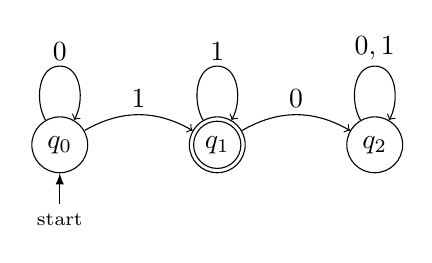
\begin{tikzpicture}

  \node[circle, draw=black] (start) at (0,0) {$q_0$};
  \node[circle, draw=black] (end) at (2,0) {$q_1$};
  \node[circle, draw=black] (sad) at (4,0) {$q_2$};

  \draw[-latex] (0,-.75) -- (start) node[below, at start]
  {\scriptsize start};

  \draw (end) circle (.3);

  \draw[->] (start) to[bend left=30] (end);
  \draw[->] (end) to[bend left=30] (sad);

  \node[above, yshift=1em] (d01l) at ($.5*(start) + .5*(end)$) {$1$};
  \node[above, yshift=1em] (d01l) at ($.5*(end) + .5*(sad)$) {$0$};



  \draw[->] (start) to[out=120, in=180] ++(0,1) to[out=0, in=60] (start);
  \node[above, yshift=1em] (d00l) at ($(start) + (0,.6)$) {$0$};

  \draw[->] (end) to[out=120, in=180] ++(0,1) to[out=0, in=60] (end);
  \node[above, yshift=1em] (d11l) at ($(end) + (0,.6)$) {$1$};

  \draw[->] (sad) to[out=120, in=180] ++(0,1) to[out=0, in=60] (sad);
  \node[above, yshift=1em] (d201l) at ($(sad) + (0,.6)$) {$0,1$};




\end{tikzpicture}
\end{document}
